\documentclass[11pt,a4paper,openany]{ctexrep}
\usepackage[a4paper,margin=23mm,headheight=15pt]{geometry}
\usepackage{amsmath,amssymb,mathtools,bm}
\usepackage{siunitx}
\usepackage{booktabs,tabularx,array,longtable}
\usepackage{enumitem}
\usepackage{graphicx}
\usepackage{xcolor}
\usepackage{tikz}
\usetikzlibrary{arrows.meta,positioning,shapes.geometric,calc,fit,decorations.pathmorphing}
\usepackage[most]{tcolorbox}
\usepackage{hyperref}
\usepackage{fancyhdr}
\usepackage{titlesec}
\usepackage{microtype}
\usepackage{setspace}

\definecolor{KidBlue}{HTML}{22577A}
\definecolor{KidTeal}{HTML}{2A9D8F}
\definecolor{KidGold}{HTML}{E9C46A}
\definecolor{KidRed}{HTML}{C8553D}
\definecolor{KidGray}{HTML}{F3F5F7}
\definecolor{KidDark}{HTML}{263238}

\hypersetup{colorlinks=true,linkcolor=KidBlue,urlcolor=KidBlue,citecolor=KidTeal,pdftitle={KID入门讲义 v0.2},pdfauthor={ChatGPT 辅助整理}}
\setstretch{1.15}
\setlist[itemize]{leftmargin=2em,itemsep=0.25em,topsep=0.4em}
\setlist[enumerate]{leftmargin=2em,itemsep=0.25em,topsep=0.4em}
\setlength{\parindent}{2em}
\setlength{\parskip}{0.25em}

\pagestyle{fancy}
\fancyhf{}
\fancyhead[L]{KID 入门讲义 v0.2}
\fancyhead[R]{\leftmark}
\fancyfoot[C]{\thepage}
\renewcommand{\headrulewidth}{0.4pt}

\titleformat{\chapter}[display]{\bfseries\Huge\color{KidDark}}{\filleft\color{KidBlue}\fontsize{44}{44}\selectfont\thechapter}{1ex}{\titlerule\vspace{1ex}\filright}
\titleformat{\section}{\Large\bfseries\color{KidBlue}}{\thesection}{0.7em}{}
\titleformat{\subsection}{\large\bfseries\color{KidTeal}}{\thesubsection}{0.7em}{}

\newtcolorbox{goalbox}{colback=KidBlue!5,colframe=KidBlue,boxrule=0.8pt,arc=2mm,title=本节目标,fonttitle=\bfseries}
\newtcolorbox{intuitionbox}{colback=KidTeal!6,colframe=KidTeal,boxrule=0.8pt,arc=2mm,title=物理直觉,fonttitle=\bfseries}
\newtcolorbox{projectbox}{colback=KidGold!16,colframe=KidGold!80!black,boxrule=0.8pt,arc=2mm,title=映射到你的 150 GHz LEKID,fonttitle=\bfseries}
\newtcolorbox{mistakebox}{colback=KidRed!5,colframe=KidRed,boxrule=0.8pt,arc=2mm,title=常见误区,fonttitle=\bfseries}
\newtcolorbox{checkpointbox}{colback=KidGray,colframe=KidDark!55,boxrule=0.7pt,arc=2mm,title=理解检查,fonttitle=\bfseries}
\newtcolorbox{formula}[1][]{colback=white,colframe=KidBlue!75,boxrule=0.9pt,arc=1mm,#1}

\newcommand{\qp}{\mathrm{qp}}
\newcommand{\Stwentyone}{S_{21}}
\newcommand{\fzero}{f_0}
\newcommand{\Qi}{Q_i}
\newcommand{\Qc}{Q_c}
\newcommand{\Qr}{Q_r}
\newcommand{\Lk}{L_k}
\newcommand{\Lg}{L_g}


% --- Flow-chart conventions (v0.2) ---
% Solid arrows = causal/signal flow; dashed arrows = parameter influence;
% plain lines = structural/reciprocal coupling. Explicit anchors avoid arrow-box collisions.
\tikzset{
  flowbox/.style={draw=KidDark!70,rounded corners=2mm,align=center,minimum height=10mm,inner sep=4pt,font=\small,fill=white},
  flowarrow/.style={-{Stealth[length=2.3mm,width=1.7mm]},line width=0.85pt,draw=KidBlue,shorten <=1.2pt,shorten >=1.2pt},
  goldarrow/.style={-{Stealth[length=2.3mm,width=1.7mm]},line width=0.85pt,draw=KidGold!75!black,shorten <=1.2pt,shorten >=1.2pt},
  influence/.style={-{Stealth[length=2.0mm,width=1.5mm]},dashed,line width=0.7pt,draw=KidTeal!85!black,shorten <=1.0pt,shorten >=1.0pt},
  structlink/.style={line width=0.8pt,draw=KidBlue!85!black},
  dimline/.style={Stealth-Stealth,thin,draw=KidDark!75}
}

\begin{document}

\begin{titlepage}
\centering
\vspace*{2.2cm}
{\fontsize{30}{38}\selectfont\bfseries\color{KidDark} KID 入门讲义}\par
\vspace{0.5cm}
{\Large\color{KidBlue} 从“一个光子”到可读出的微波信号}\par
\vspace{1.4cm}
{\large Version 0.2 · 2026-09-04}\par
\vfill
\begin{tcolorbox}[width=0.88\textwidth,colback=KidGray,colframe=KidBlue!55,arc=3mm]
\centering
\large
这不是一本“先学完凝聚态物理再碰器件”的教材。\\[0.5em]
它采用器件设计者视角：\\[0.3em]
\textbf{先建立可运行的物理图景，再逐层补上微观理论、公式、仿真与实验。}
\end{tcolorbox}
\vfill
{\large 面向：毫米/亚毫米波 KID / LEKID 初学与器件设计}\par
\end{titlepage}

\tableofcontents
\clearpage

\chapter*{如何使用这份讲义}
\addcontentsline{toc}{chapter}{如何使用这份讲义}
这份讲义按“\textbf{物理因果链}”而不是按学科目录组织。每一章都尽量回答四个问题：
\begin{enumerate}
  \item \textbf{发生了什么？} —— 先建立可视化的物理图景；
  \item \textbf{为什么？} —— 用最少但必要的公式把直觉固定下来；
  \item \textbf{怎么测？} —— 把物理量连接到真实实验中的 $I/Q$、$\Stwentyone$、频移和噪声；
  \item \textbf{与 LEKID 设计有什么关系？} —— 把材料、几何、电磁仿真和读出重新接回同一条链。
\end{enumerate}

当前版本 v0.2 在 v0.1 的基础上重点完成三件事：
\begin{itemize}
  \item 给出整个 KID 入门学习路线；
  \item 完整建立“从光子到 $\Stwentyone$”的基础物理图景，并重绘全部流程图；
  \item 新增“动能电感”专题章，从载流子惯性推到薄膜 sheet kinetic inductance 与 $\alpha$。
\end{itemize}
后续版本会逐章增加推导、数值练习、Python notebook、Sonnet/全波仿真任务以及与你的双偏振 LEKID 项目的对应分析。

\chapter{KID 入门的总体路线图}

\section{最终要学会的不是一堆名词，而是一张闭环图}
对于一个真正能够设计、仿真和读出 KID 的研究者，知识最后应当闭合成下面这条链：

\begin{center}
\begin{tikzpicture}[node distance=9mm and 6mm]
\node[flowbox,fill=KidGold!20,minimum width=31mm] (opt) {光场与吸收\\$P_{\rm abs},\nu$};
\node[flowbox,right=of opt,minimum width=36mm] (mat) {超导态与材料响应\\$\Delta,N_{\qp},\sigma_1,\sigma_2,L_k$};
\node[flowbox,right=of mat,minimum width=31mm] (res) {GHz 谐振器\\$f_0,Q_i,Q_c$};
\node[flowbox,right=of res,minimum width=34mm] (read) {读出与灵敏度\\$S_{21},I/Q,$ NEP};
\draw[flowarrow] (opt.east)--(mat.west);
\draw[flowarrow] (mat.east)--(res.west);
\draw[flowarrow] (res.east)--(read.west);

\node[flowbox,below=12mm of opt,fill=KidGray,text width=32mm] (geom) {电磁几何\\meander / backshort\\偏振 / 吸收结构};
\node[flowbox,below=12mm of mat,fill=KidGray,text width=30mm] (proc) {材料与工艺\\$T_c,t,R_\Box$\\薄膜质量};
\node[flowbox,below=12mm of read,fill=KidGray,text width=31mm] (chain) {读出链\\耦合 / 放大\\ADC / DSP};
\draw[influence] (geom.north west) to[bend left=10] node[left,font=\scriptsize]{决定吸收} (opt.south west);
\draw[influence] (geom.north east) to[bend left=15] node[below,font=\scriptsize]{改变 $L_g,C$} (res.south west);
\draw[influence] (proc.north) -- (mat.south);
\draw[influence] (chain.north) -- (read.south);
\end{tikzpicture}
\end{center}

你最终要能够在这张图中从任意一格走到任意一格。例如：
\begin{itemize}
  \item 改变膜厚，为什么会影响吸收、$\Lk$、$Q_i$ 和 responsivity？
  \item 加 backshort，为什么主要先改变毫米波吸收，却最终体现在 GHz 读出端的 $I/Q$ 上？
  \item 为什么同样一个 $\Stwentyone$ notch，可能对应完全不同的光学效率？
\end{itemize}

\section{建议的学习模块}
\renewcommand{\arraystretch}{1.25}
\begin{tabularx}{\textwidth}{>{\bfseries}p{1.5cm} p{4.0cm} X p{2.6cm}}
\toprule
模块 & 核心主题 & 学完后应该能回答的问题 & 典型产出 \\
\midrule
M1 & 从光子到 $\Stwentyone$ & KID 到底怎样把光变成可测的 IQ 变化？ & 因果链 + 极简仿真 \\
M2 & 超导基础 & Cooper pair、能隙、准粒子到底是什么？ & BCS 最小知识集 \\
M3 & 动能电感与复电导 & 为什么超导载流子的惯性等效为电感？$\sigma_1,\sigma_2$ 如何进入器件？ & $L_k$ 推导 + MB 框架 \\
M4 & 微波谐振器 & $Q_i,Q_c,Q_r$、耦合和 IQ 圆分别意味着什么？ & resonator fitting \\
M5 & 光学响应 & 光功率如何映射为 $\Delta f_0$、相位和幅度？ & responsivity 模型 \\
M6 & 噪声与 NEP & 什么时候是 photon-noise limited？TLS、GR、放大器噪声如何比较？ & noise budget \\
M7 & LEKID 电磁设计 & meander 为什么既是 absorber 又是 inductor？IDC、偏振、backshort 如何设计？ & 参数化像素模型 \\
M8 & 阵列与读出 & 如何频分复用数百/数千像素？tone spacing、动态范围如何约束设计？ & readout budget \\
M9 & 仿真与实验 & Sonnet/CST/测量数据各自验证哪一层物理？ & 仿真-测量闭环 \\
M10 & 研究课题化 & 如何从“能工作的 KID”走向可发表的问题？ & 论文问题与验证矩阵 \\
\bottomrule
\end{tabularx}

\section{推荐学习顺序}
不建议一上来死磕 Mattis--Bardeen 积分。更高效的顺序是：
\[
\boxed{
\text{可视化因果链}
\rightarrow
\text{等效电路}
\rightarrow
\text{最小超导理论}
\rightarrow
\text{复电导}
\rightarrow
\text{噪声与光学}
\rightarrow
\text{LEKID 工程设计}
}
\]
这使得每一个新公式都有“它为什么值得学”的位置。

\chapter{从一个光子到 $S_{21}$：KID 的第一性物理图景}

\begin{goalbox}
学完本章后，你应该能不看资料独立讲清：
\begin{enumerate}
  \item 为什么毫米波/亚毫米波光子能够改变超导薄膜；
  \item 为什么这种变化会改变 kinetic inductance 和 microwave loss；
  \item 为什么谐振频率与品质因数因此改变；
  \item 为什么实验最终读到的是 $\Stwentyone=I+jQ$；
  \item 一颗 LEKID 为什么可以同时扮演“光学吸收器”和“GHz 微波谐振器”。
\end{enumerate}
\end{goalbox}

\section{先看全局：KID 是一台“两种频率协同工作”的机器}
KID 初学时最容易混淆的一点，是把“被探测的光”和“用于读出的微波”混为一谈。事实上，它们通常相差几十到上百倍频率。

\begin{center}
\begin{tikzpicture}[node distance=8mm and 9mm]
% Optical / physical-state lane
\node[flowbox,fill=KidGold!23,minimum width=29mm] (ph) {信号辐射\\例如 \SI{150}{GHz}};
\node[flowbox,fill=KidGold!13,right=of ph,minimum width=31mm] (abs) {meander 薄膜\\吸收能量};
\node[flowbox,fill=KidTeal!10,right=of abs,minimum width=31mm] (qp) {$N_{\qp}\uparrow$\\超导态改变};
\node[flowbox,fill=KidBlue!8,right=of qp,minimum width=31mm] (state) {$L_k,Q_i,f_0$\\谐振器状态改变};
\draw[goldarrow] (ph.east)--(abs.west);
\draw[goldarrow] (abs.east)--(qp.west);
\draw[flowarrow] (qp.east)--(state.west);

% Microwave readout lane
\node[flowbox,fill=KidGray,below=18mm of ph,minimum width=29mm] (probe) {GHz probe\\tone source};
\node[flowbox,fill=KidBlue!6,right=of probe,minimum width=34mm] (device) {feedline + KID\\测量 $S_{21}$};
\node[flowbox,fill=KidGray,right=of device,minimum width=31mm] (adc) {低噪声放大\\ADC / DDC};
\node[flowbox,fill=KidBlue!8,right=of adc,minimum width=31mm] (iq) {$I(t),Q(t)$\\数字时间序列};
\draw[flowarrow] (probe.east)--(device.west);
\draw[flowarrow] (device.east)--(adc.west);
\draw[flowarrow] (adc.east)--(iq.west);
\draw[influence] (state.south) -- node[right,font=\scriptsize]{决定 $S_{21}(f)$} (device.north);
\end{tikzpicture}
\end{center}

一句话概括：
\begin{formula}
\[
\boxed{
P_{\rm opt}
\rightarrow N_{\qp}
\rightarrow (L_k,Q_i)
\rightarrow (f_0,Q_r)
\rightarrow S_{21}
\rightarrow I,Q
}
\]
\end{formula}

\begin{intuitionbox}
\textbf{信号光子负责“改变器件”，GHz 探针微波负责“询问器件”。}\\
KID 的巧妙之处，不是把毫米波直接送进 GHz ADC，而是让毫米波先改变一个非常灵敏的超导谐振器，再用微波精确测量这个变化。
\end{intuitionbox}

\section{第一站：入射光子必须有足够的能量}

\subsection{光子的能量尺度}
一个频率为 $\nu$ 的光子能量为
\[
E_\gamma=h\nu.
\]
对于 \SI{150}{GHz}：
\[
E_\gamma = h\nu \approx \SI{9.94e-23}{J}\approx \SI{0.620}{meV}.
\]
这个数本身没有意义，直到我们把它与超导体的能隙 $\Delta$ 比较。

\subsection{超导能隙与 pair-breaking threshold}
在弱耦合 BCS 近似下，零温能隙约为
\[
\Delta(0)\approx1.764\,k_B T_c.
\]
破坏一个 Cooper pair 至少需要产生两个准粒子，因此阈值为
\[
\boxed{h\nu\ge 2\Delta.}
\]
对应的 pair-breaking frequency 近似为
\[
\nu_{\rm pb}=\frac{2\Delta}{h}\approx \SI{73.5}{GHz/K}\times T_c.
\]

\begin{projectbox}
若取铝 $T_c\approx\SI{1.2}{K}$，则
\[
\nu_{\rm pb}\approx\SI{88}{GHz}.
\]
你的目标频率约为 \SI{150}{GHz}，明显高于这个阈值。因此从最基本的能量条件看，\SI{150}{GHz} 光子具备直接 pair breaking 的能力。
\end{projectbox}

\begin{mistakebox}
“光子能量大于 $\Delta$ 就能打碎 Cooper pair”是不准确的。一个 pair 被破坏后对应两个准粒子激发，因此最基本阈值是 $2\Delta$，不是 $\Delta$。
\end{mistakebox}

\section{第二站：Cooper pair 被破坏，准粒子数量上升}

\subsection{现在只需要一个最小的超导图景}
本章暂时不从 BCS 波函数开始。只保留三类对象：
\begin{itemize}
  \item \textbf{Cooper-pair condensate}：超导凝聚态，承担无直流电阻的集体输运；
  \item \textbf{energy gap $\Delta$}：从凝聚态激发出准粒子需要跨越的能量尺度；
  \item \textbf{quasiparticle（准粒子）}：超导体系的激发态，可以参与微波耗散并改变复电导。
\end{itemize}

当一个满足 $h\nu>2\Delta$ 的光子被薄膜吸收后，最简图景是
\[
\gamma + \text{Cooper pair}\rightarrow \qp+\qp.
\]
真实过程还包括高能准粒子的弛豫、声子产生以及二次 pair breaking，因此一个高能光子的能量最终可能形成多个低能准粒子。后续章节会用 pair-breaking efficiency $\eta$ 描述这个过程。

\subsection{为什么天文 LEKID 更适合用“光功率”而不是“一颗光子”思考}
对于连续背景与天文辐射，更合适的动力学图像是
\[
\frac{dN_{\qp}}{dt}=G-R,
\]
其中 $G$ 是准粒子生成率，$R$ 是复合率。持续光照增强通常意味着
\[
P_{\rm opt}\uparrow \Rightarrow G\uparrow \Rightarrow N_{\qp}\uparrow.
\]
因此，本讲义后续更常使用
\[
\boxed{P_{\rm opt}\rightarrow N_{\qp}}
\]
而不是把 LEKID 简化成单光子计数器。

\section{第三站：为什么准粒子增加会影响 kinetic inductance？}

\subsection{先把“动能电感”理解成惯性}
电流意味着载流子有定向运动。载流子有质量，因此它们建立和改变速度需要能量。对于交流电流，这部分能量会周期性地存入和释放。

从电路端看，只要一个元件表现出
\[
V\propto\frac{dI}{dt},
\]
它就具有电感型响应。超导载流子由于惯性产生的这种响应，就是 \textbf{kinetic inductance}。

在一个最简惯性模型中，取有效超导载流子密度为 $n_s$，可得到
\[
L_k\propto\frac{1}{n_s}.
\]
详细推导将在后续“动能电感”章节中完成。这里先抓住因果关系：光照破坏部分凝聚态，使有效超流密度下降，于是同样的交流电流需要更强的载流子速度响应，表现为更大的动能储能和更大的 $L_k$。

\begin{formula}
\[
\boxed{
N_{\qp}\uparrow
\quad\Longrightarrow\quad
n_s\downarrow
\quad\Longrightarrow\quad
L_k\uparrow
}
\]
\end{formula}

\subsection{几何电感与动能电感不是一回事}
KID 的总电感可以写成
\[
L=L_g+L_k.
\]
两者从端口看都像电感，但储能位置不同：

\begin{center}
\begin{tabular}{lll}
\toprule
量 & 主要储能位置 & 直觉 \\
\midrule
$C$ & 电场 & 电荷分离 \\
$L_g$ & 导体周围的磁场 & 电流建立磁场 \\
$L_k$ & 超导载流子的集体动能 & 载流子具有惯性 \\
\bottomrule
\end{tabular}
\end{center}

定义 kinetic inductance fraction
\[
\boxed{\alpha\equiv\frac{L_k}{L_g+L_k}.}
\]
它告诉我们总电感中有多大比例来自对超导态敏感的那部分。$\alpha$ 越大，材料状态变化越容易转化为谐振频率变化；但这并不意味着设计时应无限追求更大的 $\alpha$，因为损耗、非线性、$Q_i$ 和噪声会共同约束器件。

\section{第四站：$L_k$ 的变化如何变成谐振频率变化？}
LEKID 是一个 lumped-element resonator。最简模型为
\[
\boxed{f_0=\frac{1}{2\pi\sqrt{LC}}.}
\]
若光照主要改变 $L_k$ 而几何电感和电容在一阶近似下不变，则
\[
\frac{\delta f_0}{f_0}=-\frac{1}{2}\frac{\delta L}{L}.
\]
又因为
\[
\delta L=\delta L_k,
\]
并利用 $\alpha=L_k/L$，得到
\begin{formula}
\[
\boxed{
\frac{\delta f_0}{f_0}
=-\frac{\alpha}{2}\frac{\delta L_k}{L_k}.
}
\]
\end{formula}
因此最常见的方向是
\[
L_k\uparrow \quad\Rightarrow\quad f_0\downarrow.
\]
这就是“光照使 resonance 向低频移动”的最基础来源。

\begin{checkpointbox}
如果 $L_k$ 占总电感的比例只有 $1\%$，即使 $L_k$ 本身变化明显，总 $L$ 的变化也会被 $L_g$ 稀释。这个事实正是 $\alpha$ 在 KID 设计中如此重要的原因。
\end{checkpointbox}

\section{第五站：准粒子不仅改电感，也会增加耗散}
只看 $L_k$ 还不完整。准粒子数量增加通常也会增强 microwave dissipation，使内部品质因数下降：
\[
N_{\qp}\uparrow\Rightarrow \text{loss}\uparrow\Rightarrow Q_i\downarrow.
\]
因此光照通常同时造成：
\[
\boxed{f_0\text{ 改变}\quad +\quad Q_i\text{ 改变}.}
\]

更微观地，超导薄膜在微波频率下用复电导描述：
\[
\boxed{\sigma=\sigma_1-i\sigma_2.}
\]
在常用约定下，可以先把它记成：
\begin{itemize}
  \item $\sigma_1$：与耗散相关；
  \item $\sigma_2$：与感性/超流响应相关。
\end{itemize}
光照引起的 $N_{\qp}$ 变化会同时改变 $\sigma_1$ 和 $\sigma_2$。这就是以后 Mattis--Bardeen 理论要把“频移”和“损耗变化”统一起来的地方。

\section{第六站：实验为什么最终测 $S_{21}$？}

\subsection{把谐振器挂在一条 microwave feedline 上}
KID 通常通过耦合结构连接到微波传输线。读出系统发送一个 GHz 微波信号，并测量传输系数
\[
\boxed{S_{21}(f)=\frac{V_{\rm out}}{V_{\rm in}}.}
\]
对于最简 notch resonator，可写成
\[
S_{21}(f)=1-\frac{Q_r/Q_c}{1+2jQ_r\dfrac{f-f_0}{f_0}},
\]
并有
\[
\boxed{\frac{1}{Q_r}=\frac{1}{Q_i}+\frac{1}{Q_c}.}
\]
这里：
\begin{itemize}
  \item $Q_i$：内部损耗决定的品质因数；
  \item $Q_c$：与 feedline 耦合强弱决定的品质因数；
  \item $Q_r$：实际观测到的 loaded quality factor。
\end{itemize}

\subsection{扫频阶段：先找到谐振器}
扫过谐振频率时，$|S_{21}|$ 出现 notch。光照改变 $f_0$ 和 $Q_i$，所以 notch 会移动并改变形状。

\begin{center}
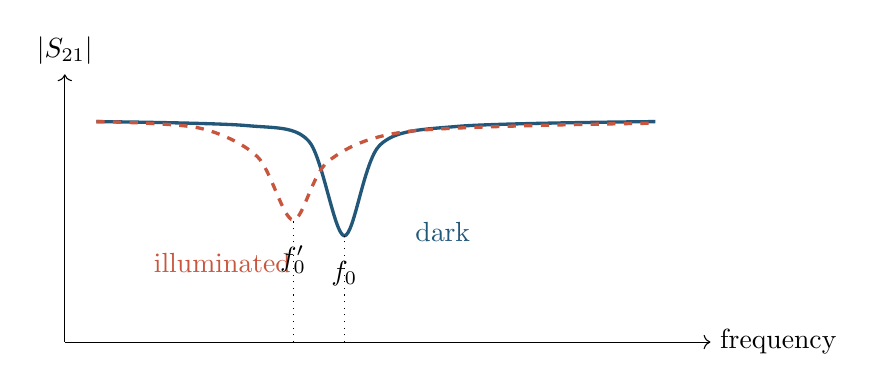
\begin{tikzpicture}[x=1cm,y=1cm]
\draw[->] (0,0)--(8.2,0) node[right]{frequency};
\draw[->] (0,0)--(0,3.4) node[above]{$|S_{21}|$};
\draw[very thick,KidBlue] plot[smooth] coordinates {(0.4,2.8)(2.3,2.75)(3.1,2.55)(3.55,1.35)(4.0,2.5)(5.0,2.74)(7.5,2.8)};
\draw[very thick,KidRed,dashed] plot[smooth] coordinates {(0.4,2.8)(1.7,2.72)(2.45,2.35)(2.9,1.55)(3.35,2.3)(4.4,2.68)(7.5,2.78)};
\node[KidBlue] at (4.8,1.4) {dark};
\node[KidRed] at (2.0,1.0) {illuminated};
\draw[dotted] (3.55,0)--(3.55,1.35) node[below,yshift=-2mm]{$f_0$};
\draw[dotted] (2.9,0)--(2.9,1.55) node[below,yshift=-2mm]{$f_0'$};
\end{tikzpicture}
\end{center}

\subsection{真正观测时：通常固定 probe tone，不需要不停扫频}
实际读出往往选取 $f_{\rm probe}\approx f_0$，持续测量一个复数：
\[
\boxed{S_{21}(t)=I(t)+jQ(t).}
\]
当谐振器因光照发生轻微移动时，固定 probe tone 在 resonance 曲线上的相对位置发生变化，因此 $I$ 和 $Q$ 随时间变化。

\begin{center}
\begin{tikzpicture}[scale=1.05]
\draw[->] (-2.6,0)--(2.8,0) node[right]{$I$};
\draw[->] (0,-2.3)--(0,2.5) node[above]{$Q$};
\draw[very thick,KidBlue] (0.35,0.05) circle (1.55);
\fill[KidBlue] (1.05,1.42) circle (2pt) node[above right]{dark operating point};
\fill[KidRed] (0.72,1.55) circle (2pt) node[above left]{illuminated};
\draw[-{Latex[length=2mm]},very thick,KidRed] (1.05,1.42)--(0.72,1.55);
\node[align=center] at (-1.4,-1.55) {扫频时形成\\近似 IQ 圆};
\end{tikzpicture}
\end{center}

这一步把 KID 与熟悉的数字接收机世界连接起来：最终进入 ADC/DSP 的不是“光子”本身，而是经过谐振器转导后的复基带响应。

\section{为什么读出微波不会自己把 Cooper pair 大量打碎？}
KID 中通常同时存在两种频率尺度：
\begin{align*}
\nu_{\rm signal} &\sim \text{几十到数百 GHz（毫米/亚毫米波）},\\
\nu_{\rm readout} &\sim \text{几百 MHz 到数 GHz（微波）}.
\end{align*}
设计上常希望
\[
h\nu_{\rm readout}<2\Delta,
\]
使单个 readout photon 的能量低于直接 pair-breaking threshold；与此同时
\[
h\nu_{\rm signal}>2\Delta,
\]
使目标光子能够被探测。

\begin{mistakebox}
“读出微波完全不影响超导态”也过于绝对。虽然单个低频 readout photon 通常不能直接 pair break，但过高读出功率仍会引起谐振器非线性、加热、准粒子分布变化等效应。因此实际系统存在最佳 readout power，而不是越大越好。
\end{mistakebox}

\section{LEKID 为什么尤其漂亮：同一块 meander 做两份工作}

\begin{center}
\begin{tikzpicture}[node distance=10mm and 13mm]
\node[flowbox,fill=KidGold!18,minimum width=31mm] (rad) {\SI{150}{GHz}\\入射辐射};
\node[flowbox,fill=KidTeal!10,right=of rad,minimum width=42mm,minimum height=16mm] (mea) {meander inductor\\毫米波 absorber\\GHz kinetic inductor};
\node[flowbox,fill=KidBlue!8,right=18mm of mea,minimum width=31mm,minimum height=16mm] (idc) {IDC\\capacitor};
\draw[goldarrow] (rad.east)--node[above,font=\scriptsize]{光学吸收} (mea.west);
\draw[structlink] (mea.east)--(idc.west);
\node[draw=KidBlue!45,rounded corners=3mm,inner sep=4mm,fit=(mea)(idc),label={[font=\scriptsize,text=KidBlue]above:同一个 GHz LC resonator}] (resgroup) {};

\node[flowbox,fill=KidGray,below=17mm of idc,minimum width=34mm] (cpl) {耦合结构\\$Q_c$};
\node[flowbox,fill=KidGray,left=of cpl,minimum width=42mm] (feed) {feedline\\GHz probe $\rightarrow$ output};
\draw[structlink,dashed] (cpl.north)--node[right,font=\scriptsize]{互易耦合} (resgroup.south east);
\draw[structlink] (feed.east)--(cpl.west);
\end{tikzpicture}
\end{center}

在 LEKID 中，lumped inductor 的 meander 往往同时承担：
\begin{enumerate}
  \item \textbf{毫米波/亚毫米波 absorber}：入射场在图形化薄膜中驱动高频电流并沉积能量；
  \item \textbf{GHz resonator 的电感}：其 $L_g+L_k$ 与 IDC 共同决定微波共振。
\end{enumerate}
因此，毫米波光学设计和 GHz 谐振器设计并不是两个独立问题；它们通过同一块超导薄膜耦合在一起。

\begin{projectbox}
对你的双偏振直接吸收 LEKID，今后每次看一个几何结构都可以问两个问题：\\
\textbf{光学问题：}它如何改变 \SI{150}{GHz} 场、电流分布、吸收和偏振选择性？\\
\textbf{读出问题：}它如何改变 $L_g$、$L_k$、$C$、$f_0$、$Q_i$、$Q_c$ 和可读出性？\\
这两个视角同时成立，才算真正理解 LEKID 几何设计。
\end{projectbox}

\section{把全章压缩成一张“因果链地图”}

\begin{center}
\begin{tikzpicture}[node distance=6mm and 13mm]
\node[flowbox,fill=KidGold!18,minimum width=58mm] (a) {$h\nu>2\Delta$\\信号功率被超导薄膜吸收};
\node[flowbox,below=of a,minimum width=58mm] (b) {Cooper pairs 被激发/破坏\\$N_{\qp}\uparrow$};
\node[flowbox,below=of b,minimum width=58mm] (c) {复电导与表面阻抗改变\\$\sigma_1,\sigma_2$ 改变};
\node[flowbox,fill=KidTeal!8,below left=8mm and 7mm of c,minimum width=45mm] (d1) {感性支路\\$L_k\uparrow$};
\node[flowbox,fill=KidTeal!8,below right=8mm and 7mm of c,minimum width=45mm] (d2) {耗散支路\\loss$\uparrow$, $Q_i\downarrow$};
\node[flowbox,fill=KidBlue!7,below=22mm of c,minimum width=66mm] (e) {谐振器响应改变\\$f_0$ 移动，notch 宽度/深度改变};
\node[flowbox,fill=KidBlue!7,below=of e,minimum width=66mm] (f) {固定 GHz probe tone\\所见 $S_{21}(t)$ 改变};
\node[flowbox,fill=KidGray,below=of f,minimum width=66mm] (g) {$I(t),Q(t)$\\数字后端估计光学信号};
\draw[flowarrow] (a.south)--(b.north);
\draw[flowarrow] (b.south)--(c.north);
\draw[flowarrow] (c.south west) to[out=-90,in=90] (d1.north);
\draw[flowarrow] (c.south east) to[out=-90,in=90] (d2.north);
\draw[flowarrow] (d1.south) to[out=-90,in=155] (e.north west);
\draw[flowarrow] (d2.south) to[out=-90,in=25] (e.north east);
\draw[flowarrow] (e.south)--(f.north);
\draw[flowarrow] (f.south)--(g.north);
\end{tikzpicture}
\end{center}

\section{本章的“公式阶梯”}
第一遍学习只需要按下面顺序记忆，不需要同时掌握所有微观细节。

\begin{enumerate}
  \item 光子能量：
  \[
  E_\gamma=h\nu.
  \]
  \item Pair-breaking threshold：
  \[
  h\nu\ge2\Delta,
  \qquad
  \Delta(0)\approx1.764k_BT_c.
  \]
  \item 动能电感的核心比例关系：
  \[
  L_k\propto\frac1{n_s}.
  \]
  \item LC resonance：
  \[
  f_0=\frac1{2\pi\sqrt{LC}},\qquad L=L_g+L_k.
  \]
  \item 小信号频移：
  \[
  \frac{\delta f_0}{f_0}=-\frac{\alpha}{2}\frac{\delta L_k}{L_k}.
  \]
  \item 品质因数关系：
  \[
  \frac1{Q_r}=\frac1{Q_i}+\frac1{Q_c}.
  \]
  \item 实验读出量：
  \[
  S_{21}=I+jQ.
  \]
\end{enumerate}

\section{六个最容易形成的错误直觉}
\begin{enumerate}
  \item \textbf{“KID 直接测光子的电信号。”}\\
  不对。光先改变超导材料，再改变谐振器，最后才改变微波传输。
  \item \textbf{“只要 $h\nu>\Delta$ 就可以 pair break。”}\\
  基本阈值应是 $2\Delta$。
  \item \textbf{“Kinetic inductance 就是导线弯弯曲曲形成的电感。”}\\
  不对。弯曲几何主要影响 $L_g$；$L_k$ 来自超导载流子的惯性。
  \item \textbf{“光照只是让 resonance 左移。”}\\
  不完整。它通常也改变损耗和 $Q_i$。
  \item \textbf{“KID 工作时必须持续扫频。”}\\
  通常扫频用于定位与标定，真正时间序列读出常使用固定 probe tones。
  \item \textbf{“读出功率越大，SNR 一定越好。”}\\
  不对。过强驱动会进入非线性、加热或改变准粒子状态。
\end{enumerate}

\section{Day 1 的 3--4 小时任务}
如果今天只围绕这一章学习，建议按以下顺序：

\begin{tabularx}{\textwidth}{p{1.8cm} X X}
\toprule
时间 & 任务 & 完成标准 \\
\midrule
35 min & 手画“光子 $\rightarrow$ IQ”因果链，并写出每一箭头为什么成立 & 不看讲义可口述完整链条 \\
45 min & 独立重算 Al 在 $T_c=\SI{1.2}{K}$ 时的 $\Delta$、$2\Delta$ 和 $\nu_{\rm pb}$；再算 \SI{150}{GHz} 光子能量 & 能判断某个频率是否满足 pair-breaking 条件 \\
55 min & 从 $f_0=1/(2\pi\sqrt{LC})$ 推导小信号 $\delta f_0/f_0$，理解 $\alpha$ 的意义 & 推导不用背结果 \\
60 min & Python 画 notch resonator 的 $|S_{21}|$ 与 IQ 圆；令 $f_0$ 左移并比较固定 probe tone 的 $\Delta I,\Delta Q$ & 得到至少 3 张图 \\
30 min & 阅读 Day 2003 的摘要/图 1，并回看本章因果链 & 能指出论文实验的“被测量量”在哪里 \\
20 min & 闭卷回答本章 8 道题 & 至少 6 题能完整解释“为什么” \\
\bottomrule
\end{tabularx}

\section{闭卷理解检查}
\begin{checkpointbox}
不查资料，尝试回答：
\begin{enumerate}
  \item 为什么 pair-breaking threshold 是 $2\Delta$？
  \item 为什么 \SI{150}{GHz} 对 Al 是一个合理的 pair-breaking 频率，而 \SI{5}{GHz} 通常不是？
  \item $N_{\qp}$ 增加后，为什么不能只讨论 $L_k$ 而忽略 $Q_i$？
  \item $L_g$ 与 $L_k$ 的能量分别储存在什么地方？
  \item 为什么 $L_k$ 增加通常导致 $f_0$ 降低？
  \item 什么是 $Q_i,Q_c,Q_r$？
  \item 为什么实际观测可以固定 probe tone，而不必一直扫频？
  \item 用一句完整的话解释：LEKID 的 meander 为什么同时是 absorber 和 resonator inductor？
\end{enumerate}
\end{checkpointbox}

\section{本章结束后你应该拥有的“一个句子”}
如果只能保留一句话，应当是：

\begin{formula}
\centering
\Large
\textbf{KID 用高于能隙阈值的光改变超导薄膜的准粒子与复电导，再用高 $Q$ 微波谐振器把这种微小变化转成可精确测量的 $S_{21}=I+jQ$ 变化。}
\end{formula}


\chapter{动能电感：为什么“载流子的惯性”会变成一个可测的电感？}

\begin{goalbox}
这一章只解决一个核心问题：\textbf{为什么超导载流子的运动惯性可以从器件端口看成一个电感 $L_k$？}
学完后你应能：
\begin{enumerate}
  \item 从 $m\,dv/dt=qE$ 独立推到一段均匀超导条带的 $L_k$；
  \item 用能量法再次得到同一个结果，并解释“电感储能”储在哪里；
  \item 理解 London penetration depth $\lambda_L$ 与 $L_k$ 的关系；
  \item 把三维电感化成薄膜工程中常用的 sheet kinetic inductance $L_{k,\Box}$；
  \item 判断长度、线宽、膜厚、超流密度怎样改变 $L_k$，以及为什么 $\alpha$ 决定频率响应；
  \item 知道电磁仿真中把金属简单设成 PEC 时，哪一部分 KID 物理会被漏掉。
\end{enumerate}
\end{goalbox}

\section{先把“电感”拆成两种储能机制}
对于 LEKID 的一段 meander，总电感可以写成
\[
L=L_g+L_k.
\]
这两个量从端口看都满足“电流变化越快，需要的电压越大”，但物理储能位置不同。

\begin{center}
\begin{tikzpicture}[node distance=10mm and 12mm]
\node[flowbox,fill=KidBlue!6,minimum width=46mm,minimum height=18mm] (c) {$C$：电容\\能量主要储存在电场\\$U_E=\tfrac12CV^2$};
\node[flowbox,fill=KidGold!13,right=of c,minimum width=46mm,minimum height=18mm] (lg) {$L_g$：几何电感\\能量主要储存在磁场\\$U_B=\tfrac12L_gI^2$};
\node[flowbox,fill=KidTeal!10,right=of lg,minimum width=46mm,minimum height=18mm] (lk) {$L_k$：动能电感\\能量储存在载流子动能\\$U_k=\tfrac12L_kI^2$};
\end{tikzpicture}
\end{center}

\begin{intuitionbox}
“meander 弯得很多，所以它有 kinetic inductance”是错误直觉。弯折、回流路径和周围磁场首先影响 $L_g$；$L_k$ 的根源是\textbf{有质量的超导载流子被交流电场加速}。即使一根完全笔直的超导条带，也有 $L_k$。
\end{intuitionbox}

\section{第一条推导：从载流子惯性到 $V=L_k\,dI/dt$}

\subsection{步骤 1：电场使超导载流子加速}
先使用一个故意简化但非常有用的模型。令有效超导载流子的质量、电荷和数密度分别为 $m^*$、$q^*$、$n_s$。忽略散射时，沿导线方向有
\[
m^*\frac{dv}{dt}=q^*E.
\]
电流密度为
\[
J=n_s q^* v.
\]
因此
\[
\frac{dJ}{dt}=n_s q^*\frac{dv}{dt}
=\frac{n_s(q^*)^2}{m^*}E,
\]
从而
\begin{formula}
\[
\boxed{
E=\frac{m^*}{n_s(q^*)^2}\frac{dJ}{dt}
}
\]
\end{formula}

这已经具有“感性”特征：电场不是与 $J$ 本身成正比，而是与 $dJ/dt$ 成正比。

\subsection{步骤 2：从电流密度变成器件端口的电流}
考虑一段长度为 $l$、宽度为 $w$、厚度为 $t$ 的均匀条带，截面积
\[
A=wt.
\]
若电流密度近似均匀，则
\[
J=\frac{I}{A},\qquad V=El.
\]
代入上式：
\[
V=\frac{m^*l}{n_s(q^*)^2A}\frac{dI}{dt}.
\]
与普通电感定义
\[
V=L\frac{dI}{dt}
\]
逐项比较，得到最基础的 kinetic inductance：
\begin{formula}
\[
\boxed{
L_k=\frac{m^*l}{n_s(q^*)^2A}
=\frac{m^*l}{n_s(q^*)^2wt}
}
\]
\end{formula}

\subsection{关于 $2e$、$2m_e$ 与 $n_s$ 的一个重要约定}
有的教材把 $n_s$ 定义为 Cooper-pair density，此时自然使用 $q^*=2e$、$m^*\approx2m_e$；另一些教材把 $n_s$ 写成“参与超流的电子密度”，公式中则使用电子的 $e,m_e$。只要\textbf{密度定义与电荷/质量定义保持一致}，最终物理结果是一致的。初学阶段最危险的是把两套约定混用，从而凭空多出一个 2 或 4 的因子。

\section{第二条推导：用能量法检查结果}
如果前面的代数让你觉得 kinetic inductance 仍然只是“人为定义”，能量法会更直观。

体积 $Al$ 内的超导载流子总动能为
\[
U_k=\frac12(n_sAl)m^*v^2.
\]
又因为
\[
I=J A=n_sq^*vA,
\]
所以
\[
v=\frac{I}{n_sq^*A}.
\]
代回：
\[
U_k
=\frac12\frac{m^*l}{n_s(q^*)^2A}I^2.
\]
而任意等效电感的储能写作
\[
U_L=\frac12LI^2.
\]
因此再次得到
\[
\boxed{L_k=\frac{m^*l}{n_s(q^*)^2A}}.
\]

\begin{checkpointbox}
这两条推导其实在说同一件事：\textbf{建立电流需要让有质量的超导载流子获得速度，因此需要储存动能；而一个端口只要以 $\tfrac12LI^2$ 的形式储能，就会表现为电感。}
\end{checkpointbox}

\section{从公式直接读出四个工程结论}
把
\[
L_k=\frac{m^*l}{n_s(q^*)^2wt}
\]
盯着看，不做任何复杂理论，就已经可以得到：
\begin{enumerate}
  \item \textbf{条带越长，$L_k$ 越大：} $L_k\propto l$；
  \item \textbf{线越窄，$L_k$ 越大：} $L_k\propto1/w$；
  \item \textbf{膜越薄，$L_k$ 越大：} 在均匀电流近似下 $L_k\propto1/t$；
  \item \textbf{超流密度越小，$L_k$ 越大：} $L_k\propto1/n_s$。
\end{enumerate}
最后一条正是 KID 探测原理的核心接口：光照或升温使超导凝聚态被激发，$n_s$ 有效下降，于是 $L_k$ 上升。

\begin{center}
\begin{tikzpicture}[node distance=7mm and 10mm]
\node[flowbox,fill=KidGray,minimum width=32mm] (geom) {几何旋钮\\$l\uparrow,w\downarrow,t\downarrow$};
\node[flowbox,fill=KidGold!13,below=of geom,minimum width=32mm] (state) {材料/状态\\$n_s\downarrow$};
\node[flowbox,fill=KidTeal!10,right=17mm of $(geom)!0.5!(state)$,minimum width=31mm] (lk) {$L_k\uparrow$};
\node[flowbox,fill=KidBlue!7,right=7mm of lk,minimum width=36mm] (alpha) {$\alpha=\dfrac{L_k}{L_g+L_k}$\\通常增大};
\node[flowbox,fill=KidBlue!7,right=7mm of alpha,minimum width=35mm] (resp) {相同材料扰动\\产生更大 $|\delta f_0|$};
\draw[influence] (geom.east) to[bend left=12] (lk.north west);
\draw[influence] (state.east) to[bend right=12] (lk.south west);
\draw[flowarrow] (lk.east)--(alpha.west);
\draw[flowarrow] (alpha.east)--(resp.west);
\end{tikzpicture}
\end{center}

\begin{mistakebox}
“线越窄、膜越薄一定越好”同样不成立。它们虽然能提高 $L_k$ 和潜在 responsivity，却也会改变毫米波表面阻抗匹配、临界电流、非线性、工艺均匀性、损耗和 $Q_i$。KID 设计几乎总是在多目标约束下寻找平衡，而不是最大化单个参数。
\end{mistakebox}

\section{London penetration depth：把 $n_s$ 藏进一个可测的长度尺度}
London 理论把超流密度写进 penetration depth：
\[
\boxed{
\lambda_L^2=\frac{m^*}{\mu_0n_s(q^*)^2}
}
\]
于是前面的均匀电流公式立刻变成
\begin{formula}
\[
\boxed{
L_k=\mu_0\lambda_L^2\frac{l}{A}
=\mu_0\lambda_L^2\frac{l}{wt}
}
\]
\end{formula}
这让一个非常重要的物理事实变得直观：
\[
n_s\downarrow\quad\Longleftrightarrow\quad\lambda_L\uparrow\quad\Longleftrightarrow\quad L_k\uparrow.
\]

\subsection{为什么叫 penetration depth？}
在块体超导体里，微波/磁场并不会像在真空中那样任意深入，而是在表面附近一个特征深度内衰减。$\lambda_L$ 就是描述这种场穿透和超流屏蔽的长度尺度。后续进入复电导与表面阻抗时，我们会看到 $\lambda$、$\sigma_2$ 与 $L_k$ 实际上是同一感性物理的不同语言。

\section{薄膜最实用的语言：每方块动能电感 $L_{k,\Box}$}
对于 KID，我们经常面对几十纳米量级的长而窄薄膜条带。若膜足够薄，使厚度方向电流可以近似均匀，则
\[
L_k=\mu_0\lambda_L^2\frac{l}{wt}
=\left(\mu_0\frac{\lambda_L^2}{t}\right)\frac{l}{w}.
\]
定义
\begin{formula}
\[
\boxed{
L_{k,\Box}\equiv\mu_0\frac{\lambda_L^2}{t}
}
\qquad (t\ll\lambda_L\text{ 的简单 London 极限})
\]
\end{formula}
以及方块数
\[
N_\Box=\frac{l}{w},
\]
就有
\[
\boxed{L_k\approx L_{k,\Box}N_\Box.}
\]

\begin{center}
\begin{tikzpicture}[x=1cm,y=1cm]
\fill[KidTeal!10] (0,0) rectangle (7.2,1.2);
\draw[KidDark!75,line width=0.8pt] (0,0) rectangle (7.2,1.2);
\foreach \x in {1.2,2.4,3.6,4.8,6.0}{\draw[KidDark!35] (\x,0)--(\x,1.2);}
\draw[flowarrow] (-0.8,0.6)--(-0.05,0.6) node[midway,above,font=\scriptsize]{$I$};
\draw[dimline] (0,-0.35)--(7.2,-0.35) node[midway,below,font=\scriptsize]{$l$};
\draw[dimline] (7.55,0)--(7.55,1.2) node[midway,right,font=\scriptsize]{$w$};
\node[font=\small] at (3.6,1.55) {$N_\Box=l/w$：宽度为 $w$ 的“方块”串联};
\end{tikzpicture}
\end{center}

“per square” 很适合平面器件：只要保持材料、膜厚和线宽定义一致，一个长条的总动能电感主要由方块数决定。对于真实 meander，弯角处的 current crowding、邻近导线磁耦合和非均匀电流会让简单 $N_\Box$ 估算产生偏差，因此它是\textbf{手算和设计直觉工具}，不是全波仿真的替代品。

\subsection{膜不再“很薄”时怎么办？}
局域 London 模型下，更一般的表面感性可写成
\[
L_{s}\approx\mu_0\lambda\,\coth\!\left(\frac{t}{\lambda}\right).
\]
当 $t\ll\lambda$ 时，$\coth(t/\lambda)\approx\lambda/t$，便退化到
\[
L_s\approx\mu_0\frac{\lambda^2}{t}.
\]
这里先把它作为“薄膜公式有适用范围”的提醒。真实 KID 薄膜还会受 dirty limit、温度和频率影响；这些会在 Mattis--Bardeen 章节统一处理。

\section{一个数值例子：为什么“每方块几 pH”最后也能变得重要？}
这里故意选一组\textbf{示意参数}，不是在宣称某种特定 Al 薄膜的真实材料常数：
\[
\lambda_{\rm eff}=\SI{200}{nm},\qquad t=\SI{20}{nm}.
\]
则薄膜近似给出
\[
L_{k,\Box}
=\mu_0\frac{\lambda_{\rm eff}^2}{t}
\approx \SI{2.5}{pH}\,/\Box.
\]
如果一段 meander 有约 $1000$ squares，那么仅动能电感就达到
\[
L_k\sim\SI{2.5}{nH}.
\]
这个量级已经足以显著参与 GHz 谐振器总电感。真正器件中必须使用实际薄膜测得或拟合的材料参数（如 $T_c$、$R_\Box$、$\Delta$、$\lambda$）或表面阻抗；不能把这个示意数值直接代入设计。

\section{从 $L_k$ 到 $\alpha$：为什么 KID 要关心“电感里有多少是动能的”}
重新定义
\[
\boxed{
\alpha=\frac{L_k}{L_g+L_k}.
}
\]
若光学扰动主要让 $L_k$ 发生微小变化，而 $L_g$ 和 $C$ 在一阶近似下不变，则
\[
\frac{\delta f_0}{f_0}
=-\frac12\frac{\delta L}{L}
=-\frac12\frac{\delta L_k}{L_g+L_k}.
\]
乘除一个 $L_k$：
\begin{formula}
\[
\boxed{
\frac{\delta f_0}{f_0}
=-\frac{\alpha}{2}\frac{\delta L_k}{L_k}.
}
\]
\end{formula}
所以 $\alpha$ 可以理解为“材料状态变化能够进入总谐振器电感的权重”。如果 $L_g\gg L_k$，材料发生同样的相对变化，却会被大量不敏感的几何电感稀释。

\begin{checkpointbox}
设两颗谐振器的 $\delta L_k/L_k$ 完全相同：A 的 $\alpha=0.05$，B 的 $\alpha=0.5$。在忽略其他差异时，B 的相对频移约为 A 的 10 倍。这并不证明 B 的总 NEP 一定更好，但说明它的\textbf{频率转导增益}更强。
\end{checkpointbox}

\section{对你的 LEKID 几何意味着什么？}
\begin{projectbox}
对你当前的 \SI{150}{GHz} 双偏振直接吸收 LEKID，meander 的线宽、总路径长度和膜厚至少同时参与四件事：
\begin{enumerate}
  \item 决定毫米波表面电流分布和吸收匹配；
  \item 改变几何电感 $L_g$；
  \item 通过 $N_\Box$ 与薄膜参数改变 kinetic inductance $L_k$；
  \item 改变 $\alpha$，进而改变相同超导态扰动造成的 $\delta f_0/f_0$。
\end{enumerate}
所以“把 meander 线做细一点”不是单纯的 GHz 谐振频率调参，也不是单纯的毫米波吸收调参，而是在同时改动两个频率域。
\end{projectbox}

\section{一个与 Sonnet/CST 直接相关的提醒：PEC 会漏掉什么？}
如果在电磁仿真里把超导薄膜完全当作 perfect electric conductor（PEC），求解器仍然可以计算：
\begin{itemize}
  \item 几何电容和大部分 $L_g$；
  \item 电流路径、耦合、辐射和很多几何效应；
  \item 在相应模型下的毫米波场分布。
\end{itemize}
但一个理想 PEC 本身没有“载流子惯性对应的表面感抗”，因此不会自动给出真实的 superconducting $L_k$ 和相关耗散。若目标是预测真实 GHz resonance frequency、材料引起的频移或 $Q_i$，通常需要把实际超导薄膜的 sheet inductance / surface impedance / 合适的超导材料模型带入。

\begin{center}
\begin{tikzpicture}[node distance=8mm and 13mm]
\node[flowbox,fill=KidGray,minimum width=40mm] (geo) {几何模型\\meander / IDC / feedline};
\node[flowbox,fill=KidRed!5,below left=12mm and 4mm of geo,minimum width=43mm] (pec) {若金属设为 PEC\\主要得到 $L_g,C$ 与几何耦合};
\node[flowbox,fill=KidTeal!8,below right=12mm and 4mm of geo,minimum width=46mm] (sup) {若加入超导表面阻抗\\可包含 $L_k$ 与材料耗散};
\node[flowbox,fill=KidBlue!7,below=27mm of geo,minimum width=58mm] (pred) {与实测 $f_0,Q_i$ 比较\\判断几何误差还是材料模型误差};
\draw[flowarrow] (geo.south west) to[out=-90,in=90] (pec.north);
\draw[flowarrow] (geo.south east) to[out=-90,in=90] (sup.north);
\draw[flowarrow] (pec.south) to[out=-90,in=155] (pred.north west);
\draw[flowarrow] (sup.south) to[out=-90,in=25] (pred.north east);
\end{tikzpicture}
\end{center}

这也是为什么以后做“仿真--实测闭环”时，不能看到 resonance 对不上就立即把问题归咎于几何。\textbf{几何电感、电容、动能电感、材料损耗和工艺偏差都可能把 $f_0$ 推动。}

\section{这一章暂时没有做什么}
为了不把第一轮学习变成公式堆积，本章刻意没有完整推导：
\begin{itemize}
  \item BCS 中 $n_s(T)$ 与 $N_{qp}(T)$ 的严格关系；
  \item dirty-limit 超导薄膜的 $L_{k,\Box}\approx\hbar R_\Box/(\pi\Delta)$ 等常用结果；
  \item 复电导 $\sigma_1-i\sigma_2$ 与 surface impedance 的严格关系；
  \item Mattis--Bardeen 积分和有限频率、有限温度修正。
\end{itemize}
这些不是被忽略，而是被放到下一层理论中。现在先确保 $L_k$ 的物理来源已经不再神秘。

\section{本章的公式阶梯}
\begin{enumerate}
  \item 载流子动力学：
  \[
  m^*\frac{dv}{dt}=q^*E.
  \]
  \item 电流密度：
  \[
  J=n_sq^*v.
  \]
  \item 均匀条带的动能电感：
  \[
  \boxed{L_k=\frac{m^*l}{n_s(q^*)^2wt}}.
  \]
  \item London penetration depth：
  \[
  \boxed{\lambda_L^2=\frac{m^*}{\mu_0n_s(q^*)^2}}.
  \]
  \item 薄膜每方块动能电感：
  \[
  \boxed{L_{k,\Box}\approx\mu_0\frac{\lambda_L^2}{t}}.
  \]
  \item 总动能电感：
  \[
  L_k\approx L_{k,\Box}\frac{l}{w}.
  \]
  \item 动能电感占比与小信号频移：
  \[
  \boxed{\alpha=\frac{L_k}{L_g+L_k}},\qquad
  \boxed{\frac{\delta f_0}{f_0}=-\frac{\alpha}{2}\frac{\delta L_k}{L_k}}.
  \]
\end{enumerate}

\section{建议用 60--90 分钟完成的手算与代码任务}
\begin{enumerate}
  \item 不看讲义，从 $m\,dv/dt=qE$ 推到 $L_k=m^*l/[n_s(q^*)^2wt]$；
  \item 再用 $U_k=\tfrac12nmv^2V$ 独立推一次，检查两条路线是否一致；
  \item 写 10 行左右 Python：令 $L_g=8\,\mathrm{nH}$、$L_k$ 从 $0.5$ 到 $8\,\mathrm{nH}$ 扫描，画出 $\alpha$ 和 $f_0$ 的变化；
  \item 再令 $\delta L_k/L_k=10^{-4}$，画 $\alpha$ 从 0 到 1 时 $|\delta f_0/f_0|$ 的变化；
  \item 最后用一句话回答：\textbf{为什么 KID 不是“几何电感探测器”？}
\end{enumerate}

\section{闭卷理解检查}
\begin{checkpointbox}
\begin{enumerate}
  \item 一根完全笔直的超导条带有没有 kinetic inductance？为什么？
  \item $L_g$ 与 $L_k$ 分别把能量储存在哪里？
  \item 为什么 $L_k\propto1/n_s$？
  \item 把线宽减半，在最简单均匀电流模型里 $L_k$ 如何变化？
  \item 什么叫“每方块电感”？为什么 $l/w$ 没有量纲？
  \item 为什么 PEC 仿真可以给出漂亮的 resonance，却仍可能把真实 $f_0$ 算偏？
  \item $\alpha$ 大意味着什么？它为什么不是“越大越好”的单一优化目标？
\end{enumerate}
\end{checkpointbox}

\chapter*{后续版本计划}
\addcontentsline{toc}{chapter}{后续版本计划}
\begin{itemize}
  \item v0.3：Cooper pair、BCS 能隙、热准粒子与 $N_{qp}(T)$；
  \item v0.4：复电导、surface impedance 与 Mattis--Bardeen 的器件化理解；
  \item v0.5：$Q_i/Q_c/Q_r$、notch resonator、IQ circle 与实际 fitting；
  \item v0.6：optical responsivity、quasiparticle lifetime、NEP 与噪声；
  \item v0.7：LEKID absorber / IDC / coupling / polarization / backshort 的电磁设计；
  \item v0.8：把上述理论逐项映射到当前双偏振 \SI{150}{GHz} LEKID 项目与 Sonnet/CST 验证矩阵。
\end{itemize}

\chapter*{建议参考资料}
\addcontentsline{toc}{chapter}{建议参考资料}
\begin{enumerate}
  \item P. K. Day et al., ``A broadband superconducting detector suitable for use in large arrays,'' \textit{Nature}, 425, 817--821 (2003).
  \item S. Doyle, \textit{Lumped Element Kinetic Inductance Detectors}, PhD thesis, Cardiff University (2008).
  \item J. Zmuidzinas, ``Superconducting Microresonators: Physics and Applications,'' \textit{Annual Review of Condensed Matter Physics}, 3, 169--214 (2012).
  \item J. Gao, \textit{The Physics of Superconducting Microwave Resonators}, PhD thesis, California Institute of Technology (2008).
\end{enumerate}

\end{document}
